\documentclass{article}
\usepackage[utf8]{inputenc}
\usepackage{amsmath}
\usepackage{float}
\usepackage{graphicx}
\title{Power-line measurements in 116 Prospect House, Princeton University}
\author{Abhinav Narain }
\date{April 24, 2017}
\begin{document}
\maketitle
\section{Purpose}
Purpose of the document is to find how good/bad is a power-line of a
normal house. It visually compares measurements to measurements from
power-line in E-quad lab.

The measurements are from a house with no inhabitants and hence there
were no appliances or devices to be turned on for test
measurements.

\section{Conclusion} 
\begin{enumerate}
\item It is not convincing(at present) that one location is
  sufficient to detect the state of all the appliances(in the current
  experiments --light bulbs) in the house
\item The noise in home looks considerably lower than from E-quad
\end{enumerate}
\section{Measurement}
\textbf{Data Captures.} Two traces each for a duration of 30 minutes
were captured from ground floor and top (2nd) floor of the
house. These are for analysis, but at present not clear how helpful
this would be. There are shorter traces of 3 minutes that were
captured which are presented below. \\

\textbf{Experiment Design}. There was a laptop and a raspberry Pi that
were plugged into the wall-port near the measurement apparatus. Apart
from it the lighting lamps on different floors were turned on and off
at approximately 16 seconds interval to see observable differences in
the spectrograms.

\section{Results}

\subsection{Ground Floor measurements}
\begin{figure}[H]
\centering
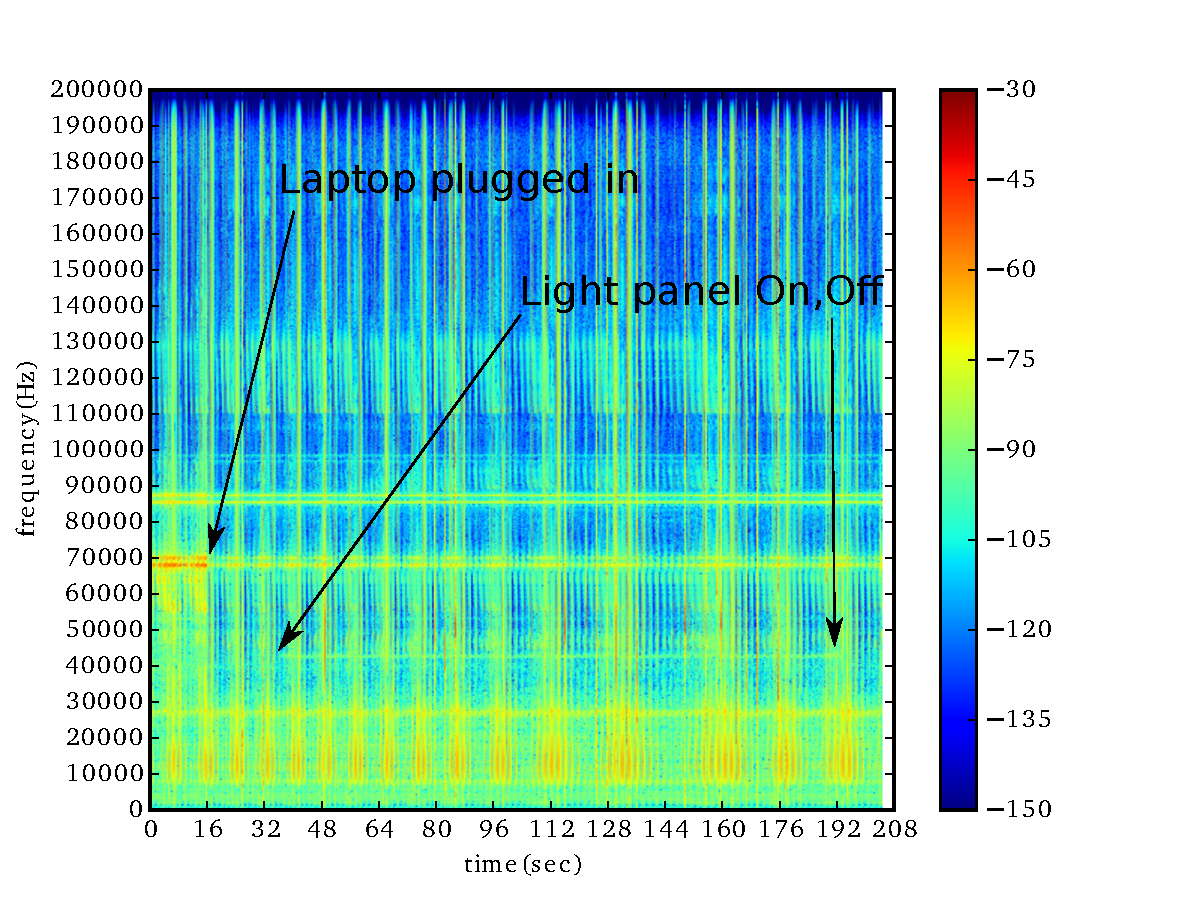
\includegraphics[width=\textwidth]{figures/EventDown_2048.pdf}
\caption{Events generated when the measurements are conducted from First
  room on the ground floor given by Table~\ref{table:ground}}
\label{fig:ground}
\end{figure}

\begin{table}
  \begin{tabular}{|l|l|l|}
    \hline 
Events & Time (On) & Time(Off) \\\hline
Laptop 					 & 16 sec & 192 \\\hline 
Ground Floor first room light panel 	 & 32	 & 176 \\\hline
Ground Floor bulb(1) 			 & 48	 & 160 \\\hline 
Ground Floor light panel		 & 64	 & 144 \\\hline 
Middle stairs bulbs(3) 			 & 72	 & 128 \\\hline 
Top Floor Stair light bulbs(2) 		 & 96	 & 112 \\\hline
\end{tabular}
\label{table:ground}
\caption{Table showing list of Events generated and time(in seconds)
  when the measurements are done on ground floor(First room) of the
  house, corresponding to Figure~\ref{fig:ground}}
\end{table}

Comments on Figure~\ref{fig:ground}:
\begin{enumerate}
\item When laptop is plugged in, there is a change in the frequency
  band of 55-85 KHz  
\item There seems to be (destructive) interference in the frequencies
  for laptop which I had not thought about. I would expect certain
  frequency to show up instead of a band of frequencies getting
  lighter in intensity as in the spectrogram  
\item Light panel switch is in the first room and powers the light in
  the room. The EMI generated is the only one that is visibly
  noticeable in the spectrogram  
\item The rest of the events in the table~\ref{table:ground} are not
  noticed in the spectrogram  
\end{enumerate}

\subsection{Top Floor Experiment}
\begin{figure}[H]
\centering
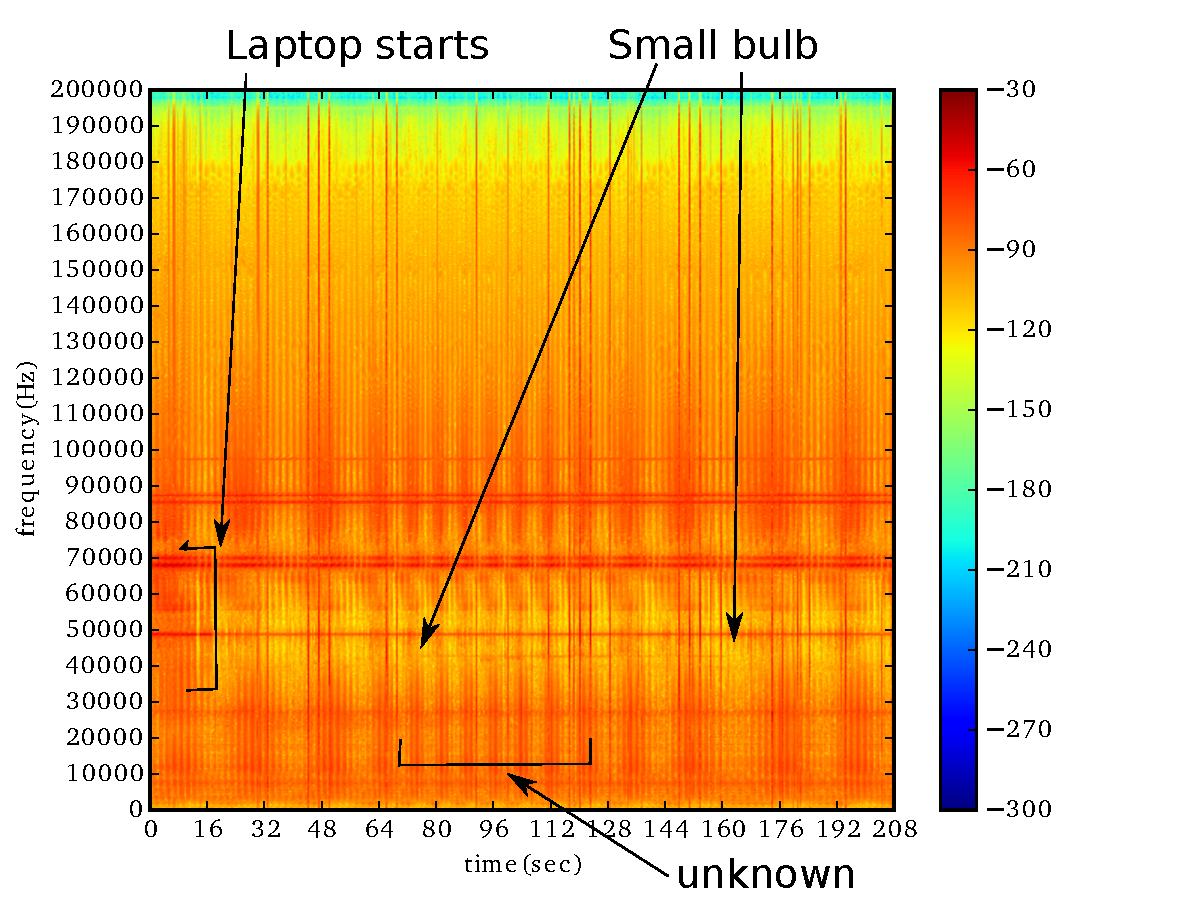
\includegraphics[width=\textwidth]{figures/EventTop_2048.pdf}
\caption{Events generated when the measurements are conducted from First
  room on the ground floor given by Table~\ref{table:top}}
\label{fig:top}
\end{figure}

\begin{table}
  \begin{tabular}{|l|l|l|}
\hline
Events &  Time (On) & Time (Off) \\\hline
Laptop 					& 16 sec & 192 \\\hline
Top floor Stair light bulbs(2) 	        & 32	 & 176 \\\hline
Middle stairs bulbs(3) 			& 48	 & 160 \\\hline
Ground Floor light panel		& 64	 & 144 \\\hline
Ground Floor bulb(1) 			& 80	 & 128 \\\hline
Ground Floor first room light panel 	& 96	 & 112 \\\hline
\end{tabular}
\label{table:top}
\caption{Table showing list of events generated and time(in seconds)
  when the measurements are done on the top floor of the
  house, corresponding to Figure~\ref{fig:top}. Bracketed number
  represents the number of bulbs turned on by single switch.}
\end{table}
Comments on Figure~\ref{fig:top}:
\begin{enumerate}
\item When laptop is plugged in, there is a change in the frequency
  band of 55-85 KHz
\item There is no observable change in EMI when other light switches
  are turned on/off
\item There is change in time period of the cyclic EMI pattern labelled
  "unknown" in the spectrogram
\item The dB scale is the same on all the spectrograms so they can be compared easily.
\end{enumerate}

\subsection{Lab Experiment}
\begin{figure}[H]
\centering
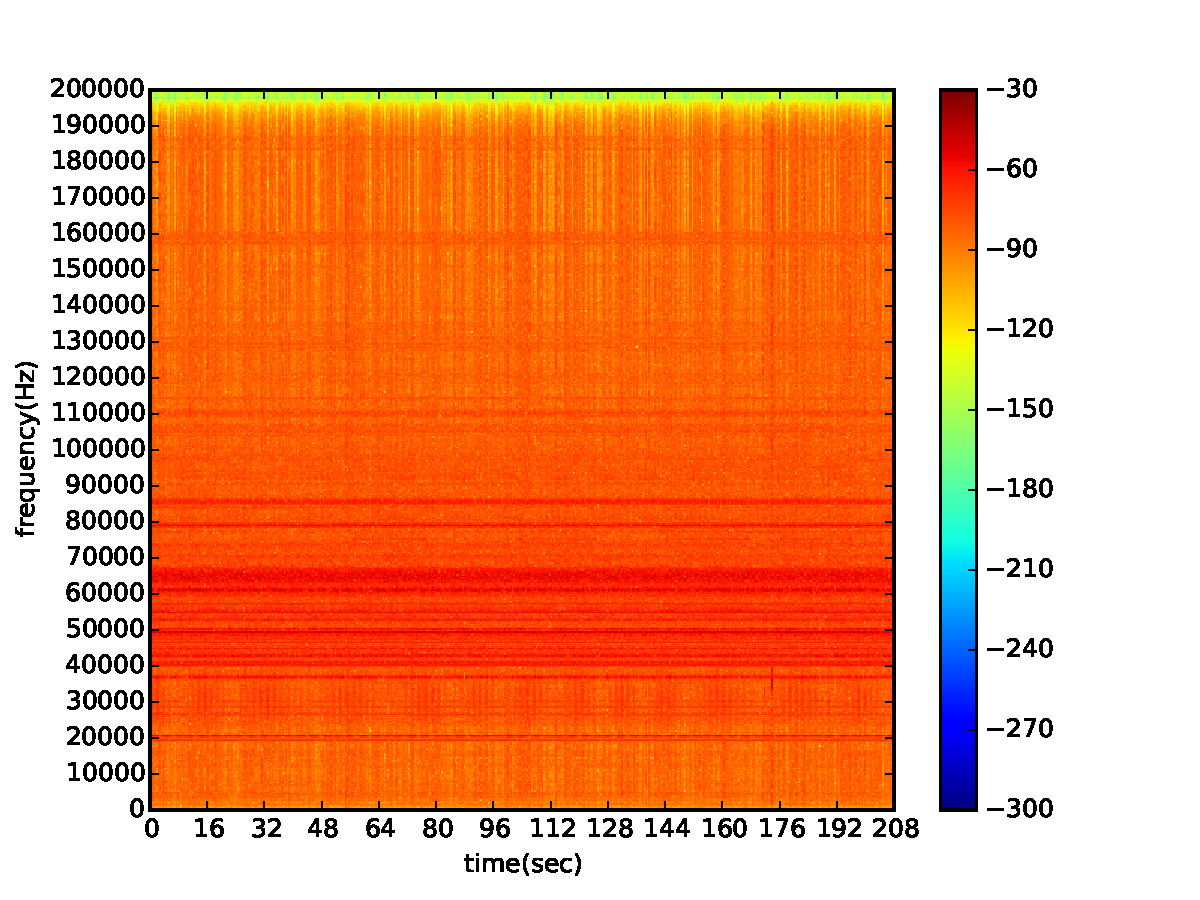
\includegraphics[width=\textwidth]{figures/labref_1_2048.pdf}
\caption{Power-line spectrum in E-Quad lab of first 200 KHz frequency band}
\label{fig:lab}
\end{figure}

\begin{enumerate}
\item The noise floor of the entire spectrum in E-Quad is higher than
  noise floor of home. No devices were turned on/off while experiment was conducted.
\item The dominant frequency around 85KHz is present in both home and E-Quad
\item The frequency band of 40 KHz to 70 KHz is cluttered. This might
  be because most of the devices have switching frequencies in the
  range and there are many high power consuming device on the line
\end{enumerate}

\section{File Sizes for data collection}
Keeping logs for the size of data collection in case researchers at
Princeton are interested in long term data captures.
\begin{enumerate}
\item For a sample rate of 400 KHz (real sampling), a file of float
  data type is saved.
\item 30 minute of data collection, the generated around \textbf{2.8
  GB} file. Similar file sizes for collection from top, ground floor
  of the house.  
\item File size grows depending on the amount of data captured instead
  of time period of capture. For example, for same time period of 200
  seconds the file generated in 200 secs at home PL is \textbf{95 MB},
  while in E-Quad EE dept, it is \textbf{385 MB}.  
\end{enumerate}
\section{Hardware Used}
The Power-line Coupler used is : Echelon Power-line Coupling
Circuit. MODEL 78200R Echelon Corporation San Jose, California. PL-20
L-E 120V
\section{References}
\end{document}
